\section{Installazione}
Il deploy e la configurazione dell'intero sistema consistono di un numero considerevole di procedure da applicare.\\
In accordo con il proponente \PROPONENTE, il quale è anche l'utilizzatore del prodotto, verranno fornite da quest'ultimo le credenziali di accesso ai servizi esterni e piattaforme elencate in \ref{configurazione}, in maniera tale che le attività di deploy e configurazione siano realizzate dal team \GRUPPO.\\
Tuttavia, viene di seguito esposto come fare il deploy e la configurazione del sistema.\\
I servizi esterni, per essere utilizzati, necessitano di alcune chiavi, le quali dovranno essere impostate nel sistema. Per fare ciò, si farà utilizzo del framework Serverless, tramite il quale verranno impostate le chiavi come variabili d'ambiente in AWS.\\
Il procedimento dettagliato verrà esposto in versioni successive di questo documento.
\subsection{Download}\label{download}
Per scaricare l'applicativo è sufficiente clonare o scaricare il repository disponibile al link \url{https://github.com/CoCodeSWE/AtAVi} (ultima visita 2017-05-07).

\subsection{Configurazione}\label{configurazione}
Per il deploy dei servizi, è necessario inizialmente installare Node.js al fine di  ottenere i moduli npm necessari alla corretta esecuzione del software. Node.js è disponibile al link \url{https://nodejs.org/en/} (ultima visita 2017-06-10).\\In secondo luogo, è necessario creare e configurare alcuni account per il corretto funzionamento del prodotto.

\subsubsection{Amazon Web Services}
\paragraph{Creazione}
Amazon Web Services è una collezione di servizi di cloud computing che compongono la piattaforma "on demand" offerta dall'azienda Amazon. Questi servizi sono operativi in 12 regioni geografiche in cui Amazon stessa ha suddiviso il globo.\\
I servizi utilizzati dal prodotto sono:
\begin{itemize}
	\item API Gateway;
	\item Simple Notification Service;
	\item Lambda;
	\item DynamoDB.
\end{itemize}
Per usufruire di essi, è sufficiente creare un account alla pagina \url{https://aws.amazon.com} (visitato in data 2017-05-02) cliccando sul pulsante "Registrazione" (figura \ref{fig:aws}). \\
Durante la registrazione, verrà chiesto di associare una carta di credito all'account. Questa operazione deve essere fatta, altrimenti non sarebbe possibile fare utilizzo dei servizi offerti.
\begin{figure}[h]
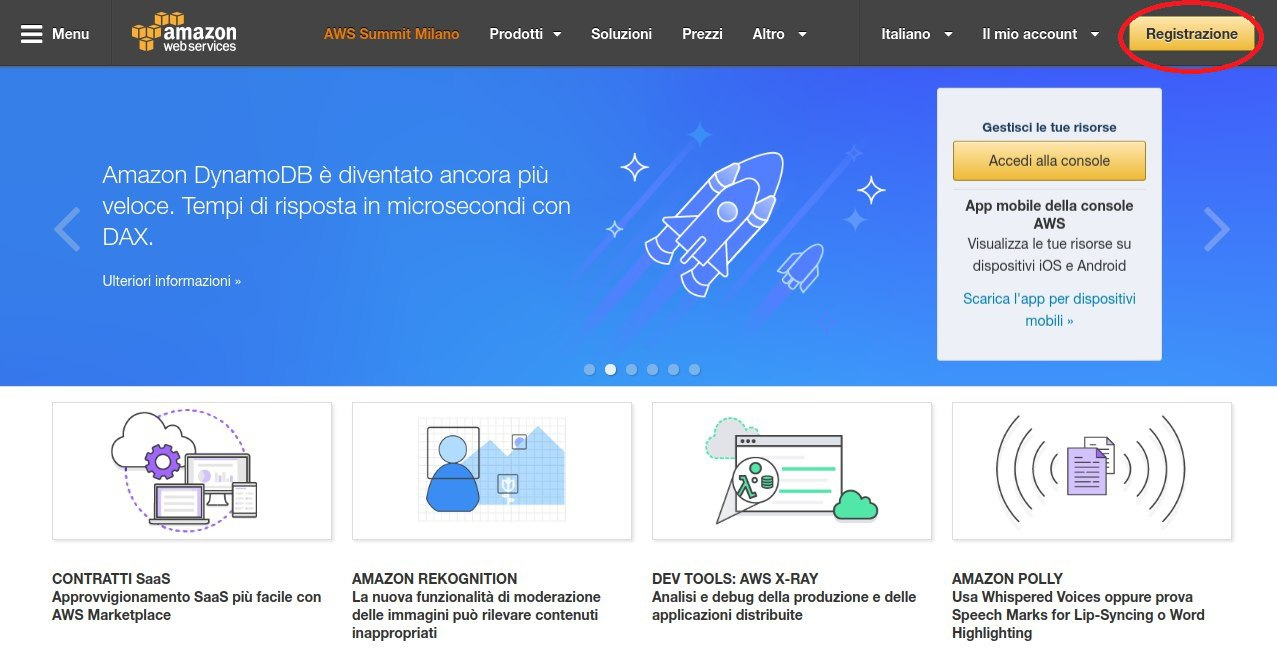
\includegraphics[width=\textwidth,height=\textheight,keepaspectratio]{sezioni/images/aws.jpg}
\caption{Registrazione AWS}\label{fig:aws}
\end{figure}
\newpage
\subsubsection{Serverless}
\paragraph{Creazione}
Serverless è un framework per alcuni servizi di cloud computing, tra i quali quelli di Amazon Web Services. È un progetto molto giovane, ma che gode già di un ottimo supporto.\\
Esso permette la realizzazione e il deploy dei servizi in maniera molto più facile e veloce, infatti l'effettivo deploy del sistema è semplificato, velocizzato e automatizzato grazie ad esso. \\
È necessario installare il framework lanciando il comando \file{npm install serverless -g} dal terminale.
\paragraph{Configurazione}
Una volta installato, è necessario applicare la seguente procedura:
\begin{itemize}
	\item creare delle AWS Access Key seguendo le istruzioni presenti al link \url{https://serverless.com/framework/docs/providers/aws/guide/credentials#creating-aws-access-keys} (visitato in data 2017-05-02);
	\item fornire le credenziali create seguendo le istruzioni al link \url{https://serverless.com/framework/docs/providers/aws/guide/credentials#setup-with-serverless-config-credentials-command} (visitato in data 2017-05-02);
\end{itemize}

\subsubsection{Microsoft Speaker Recognition}\label{speakerRec}
\paragraph{Creazione}
Questo servizio viene utilizzato per realizzare le funzionalità che richiedono il riconoscimento vocale, quali la costruzione dell'impronta vocale (\gl{enrollment}) di un nuovo amministratore e l'accesso al sistema.\\
È necessario creare un account al link \url{https://www.microsoft.com/cognitive-services} (visitato in data 2017-05-02) cliccando sul pulsante "Get started for free" (figura \ref{fig:microsoft}). Il trial gratuito ha durata di 90 giorni.
\begin{figure}[h]
	\centering{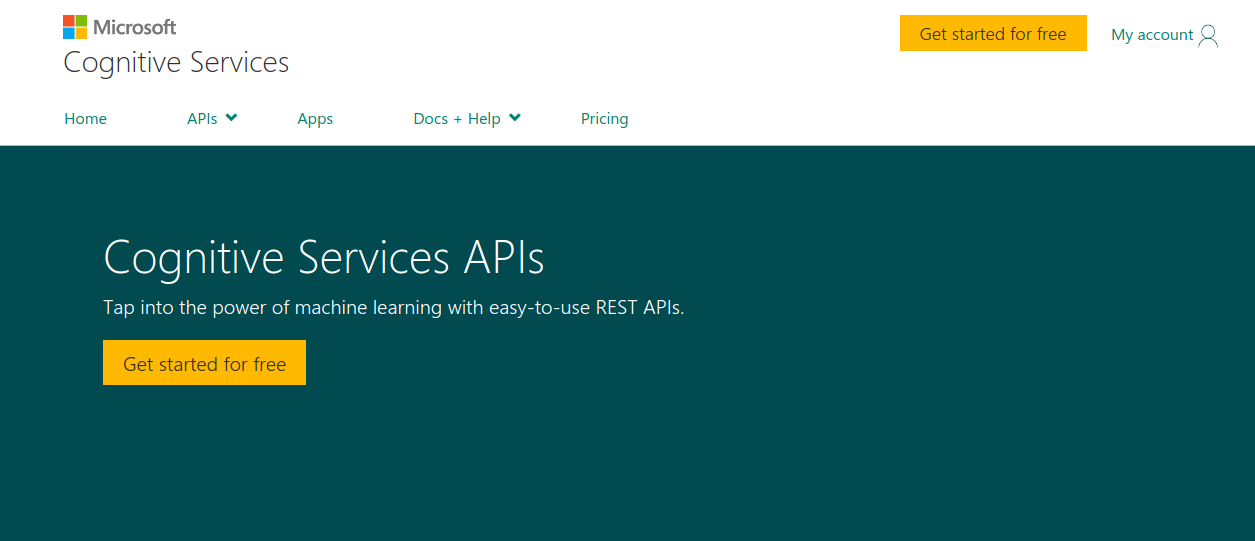
\includegraphics[width=0.8\textwidth,height=\textheight,keepaspectratio]{sezioni/images/microsoft.png}}
	\caption{Registrazione Microsoft Cognitive Services}\label{fig:microsoft}
\end{figure}
\paragraph{Configurazione}
Una volta effettuato l'accesso, è necessario applicare la seguente procedura:
\begin{itemize}
	\item tramite la pagina principale, selezionare "Subscribe to new free trials" per aggiungere un servizio (figura \ref{fig:addMicrosoft});
	\item scorrere la lista e selezionare "Speaker Recognition - Preview" e "I agree to the Microsoft Cognitive Service Terms" come in figura \ref{fig:speakerRec};
	\item tornare nella pagina principale per visualizzare le credenziali per utilizzare il nuovo servizio (figura \ref{fig:credMicrosoft});
\end{itemize}

\begin{figure}[h]
	\centering{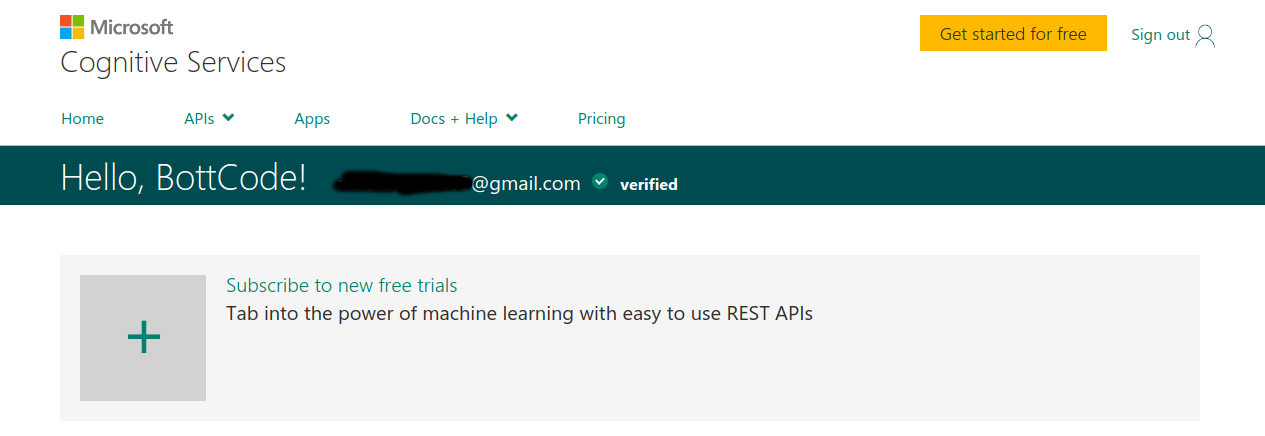
\includegraphics[width=0.8\textwidth,height=\textheight,keepaspectratio]{sezioni/images/microsoft1.png}}
	\caption{Aggiungere un servizio Microsoft}\label{fig:addMicrosoft}
\end{figure}
\begin{figure}[h]
	\centering{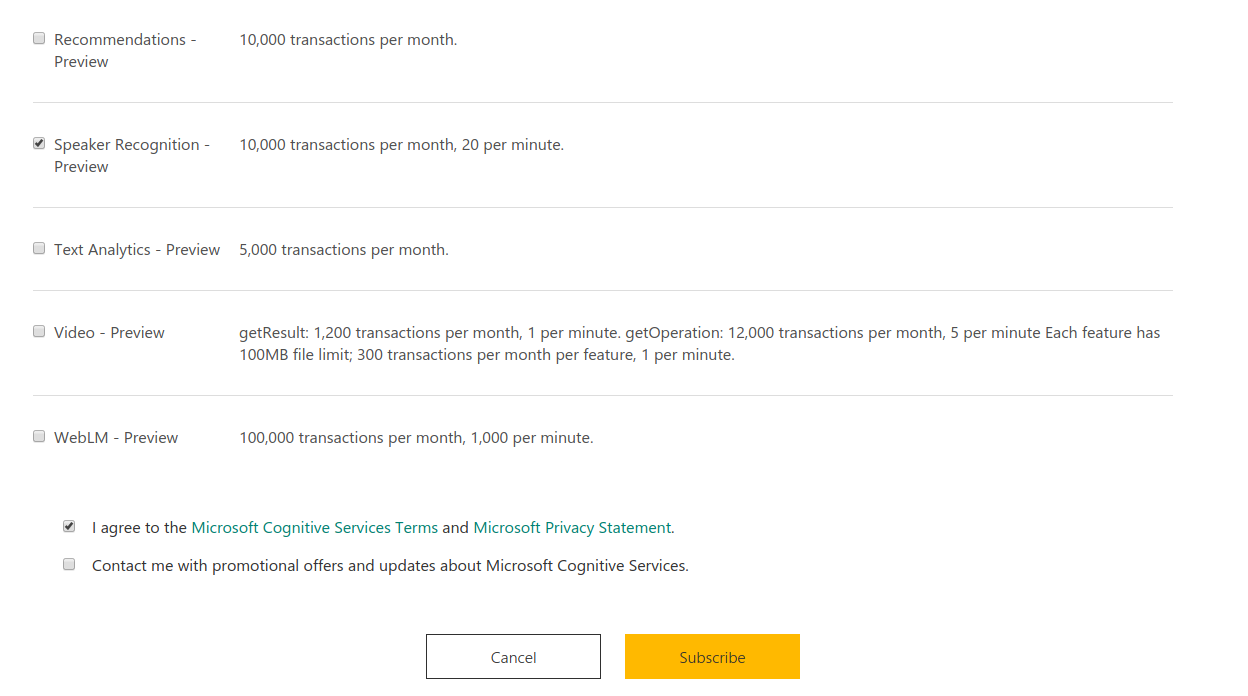
\includegraphics[width=0.8\textwidth,height=\textheight,keepaspectratio]{sezioni/images/microsoft2.png}}
	\caption{Selezionare Speaker Recognition Microsoft}\label{fig:speakerRec}
\end{figure}
\begin{figure}[h]
	\centering{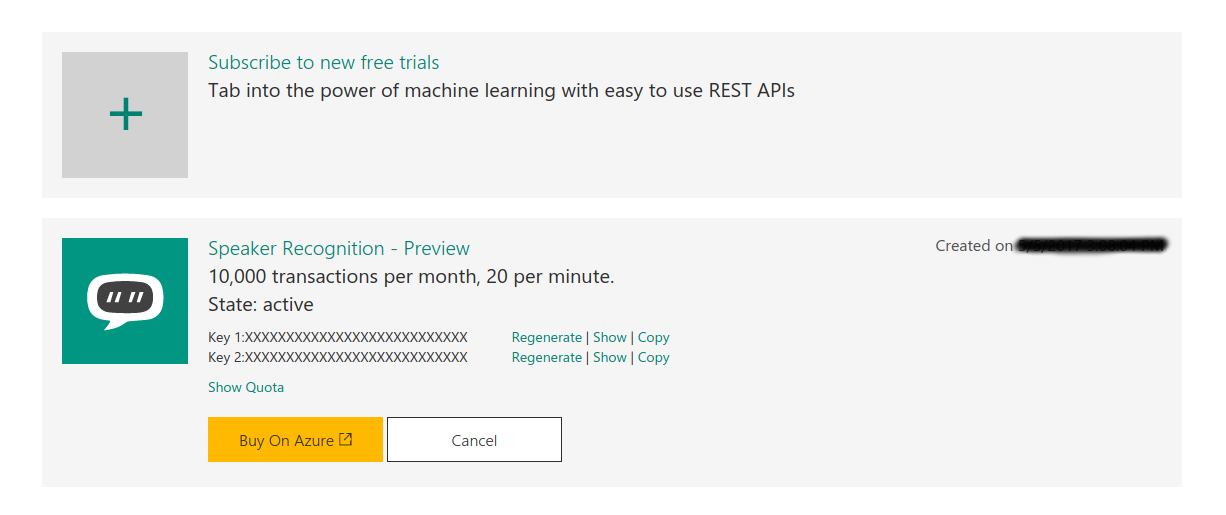
\includegraphics[width=0.8\textwidth,height=\textheight,keepaspectratio]{sezioni/images/microsoft3.png}}
	\caption{Ottenere le credenziali Speaker Recognition Microsoft}\label{fig:credMicrosoft}
\end{figure}
\newpage
\subsubsection{IBM Watson Speech to Text}
\paragraph{Creazione}
Questo servizio viene utilizzato per realizzare le funzionalità di Speech to Text, ovvero l'estrazione del testo pronunciato in un file audio.\\
È necessario creare un account su IBM Bluemix (figura \ref{fig:bluemix}) al seguente link \url{https://console.ng.bluemix.net/registration/?target=/catalog/\%3fcategory=watson} (visitato in data 2017-05-02). Vengono concessi 30 giorni di utilizzo gratuito, oltre i quali è necessario associare una carta di credito all'account.
\begin{figure}[h]
	\centering{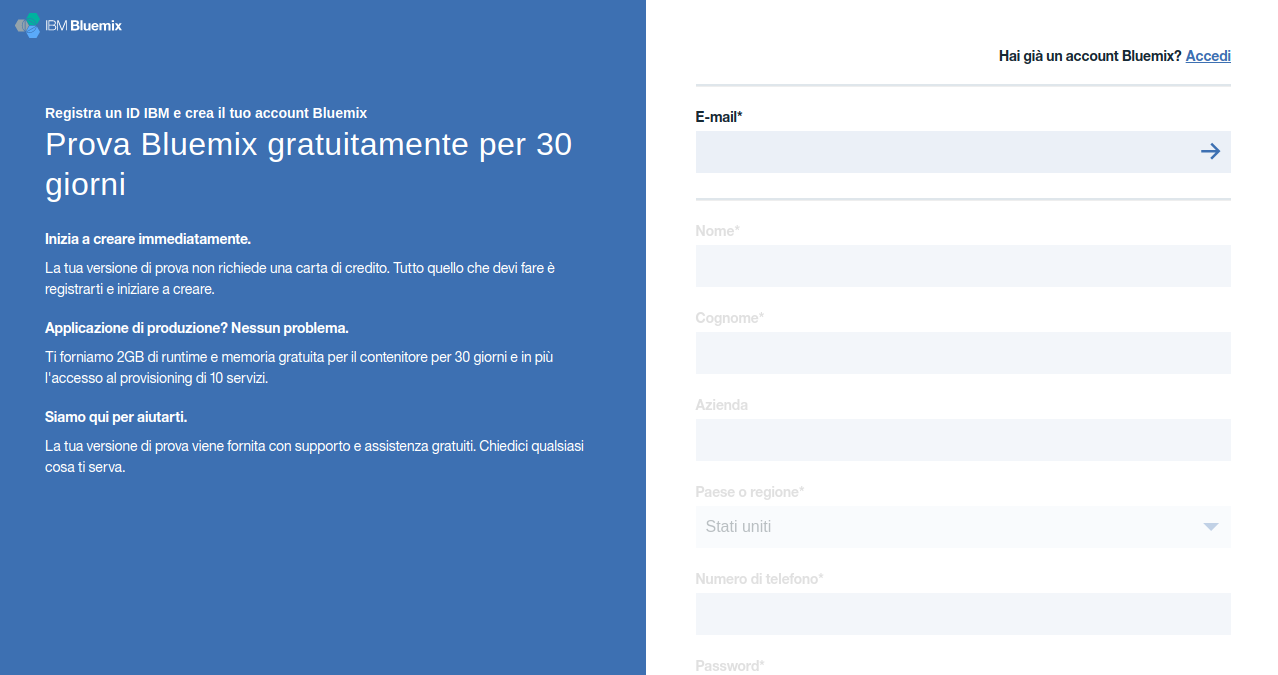
\includegraphics[width=0.8\textwidth,height=\textheight,keepaspectratio]{sezioni/images/bluemix.png}}
	\caption{Registrazione bluemix}\label{fig:bluemix}
\end{figure}
\paragraph{Configurazione}
Una volta effettuato l'accesso, è necessario applicare la seguente procedura:
\begin{itemize}
	\item accedere alla sezione dei servizi Watson \url{https://console.ng.bluemix.net/catalog/?category=watson} (visitato in data 2017-05-02) e cliccare sul servizio di Speech to Text (figura \ref{fig:consoleWatson});
	\item attivare il servizio cliccando su "Create" (figura \ref{fig:serviceWatson});
	\item Selezionare "Services" e poi "Dashboard" dal menù a sinistra, in maniera tale da ottenere la lista dei servizi attivati. Cliccare sul servizio di Speech to Text per visualizare le credenziali di utilizzo (username e password, figura \ref{fig:credentialsWatson}).
\end{itemize}

\begin{figure}[h]
	\centerline{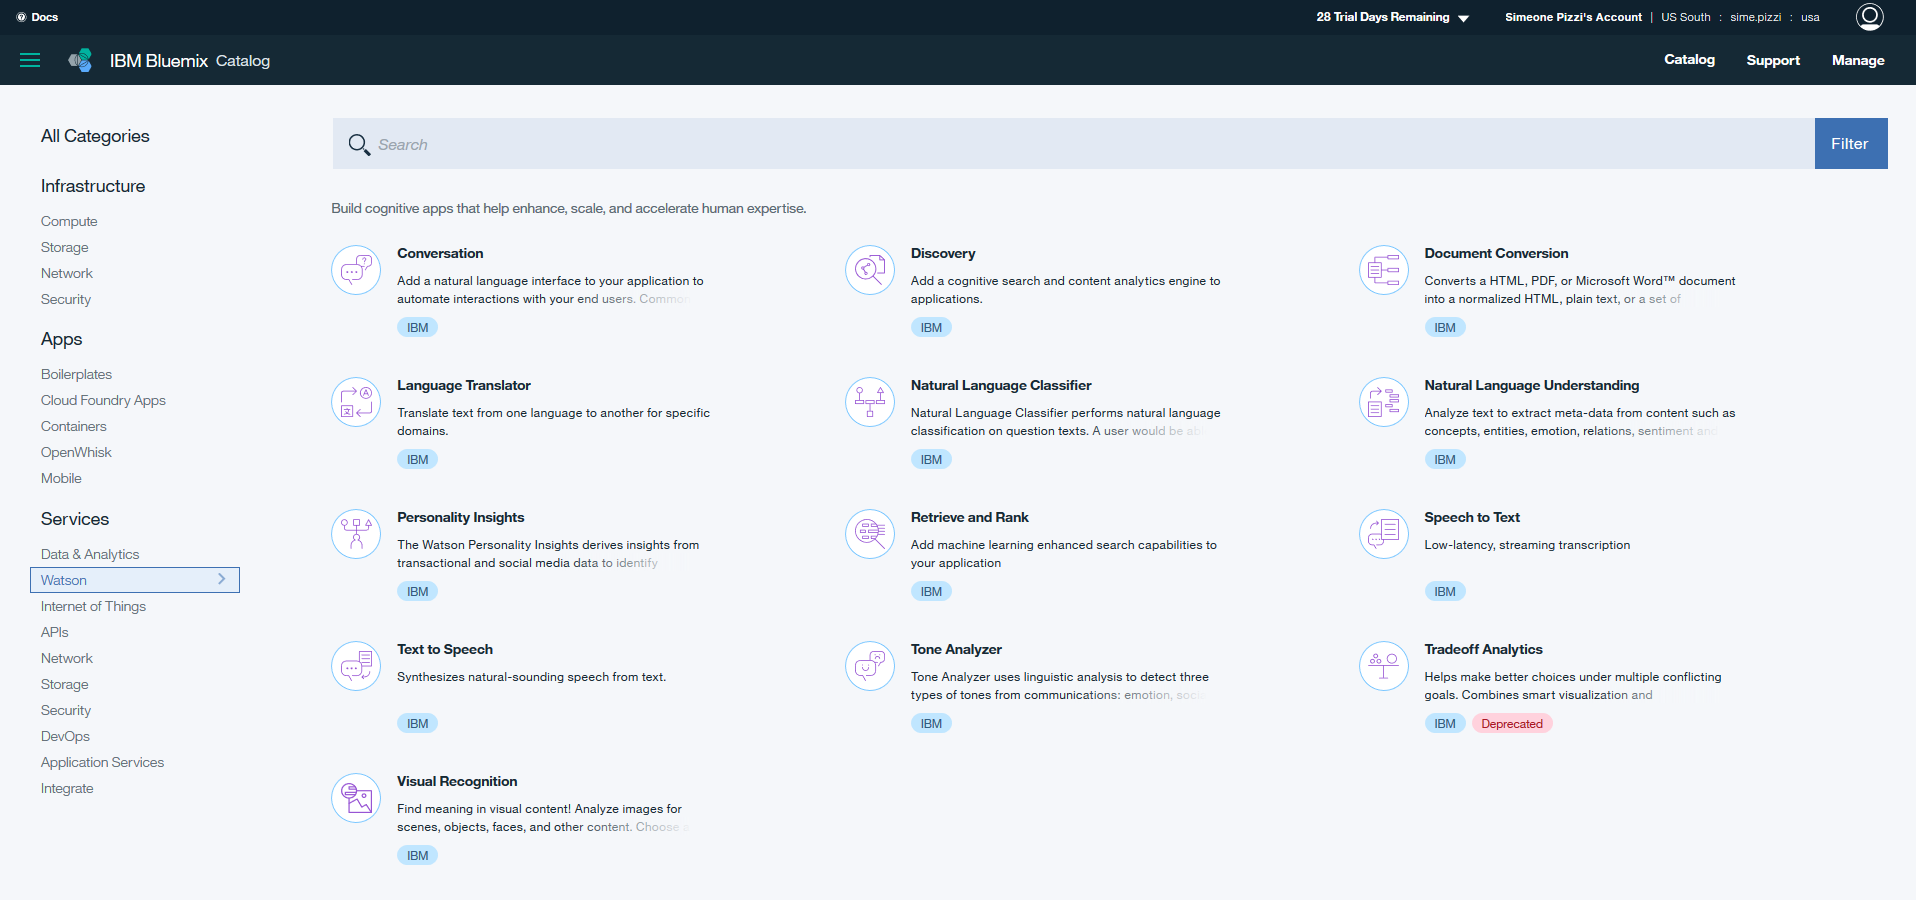
\includegraphics[width=1\textwidth,height=\textheight,keepaspectratio]{sezioni/images/watson.PNG}}
	\caption{Catalogo dei servizi IBM Watson}\label{fig:consoleWatson}
\end{figure}
\begin{figure}[h]
	\centerline{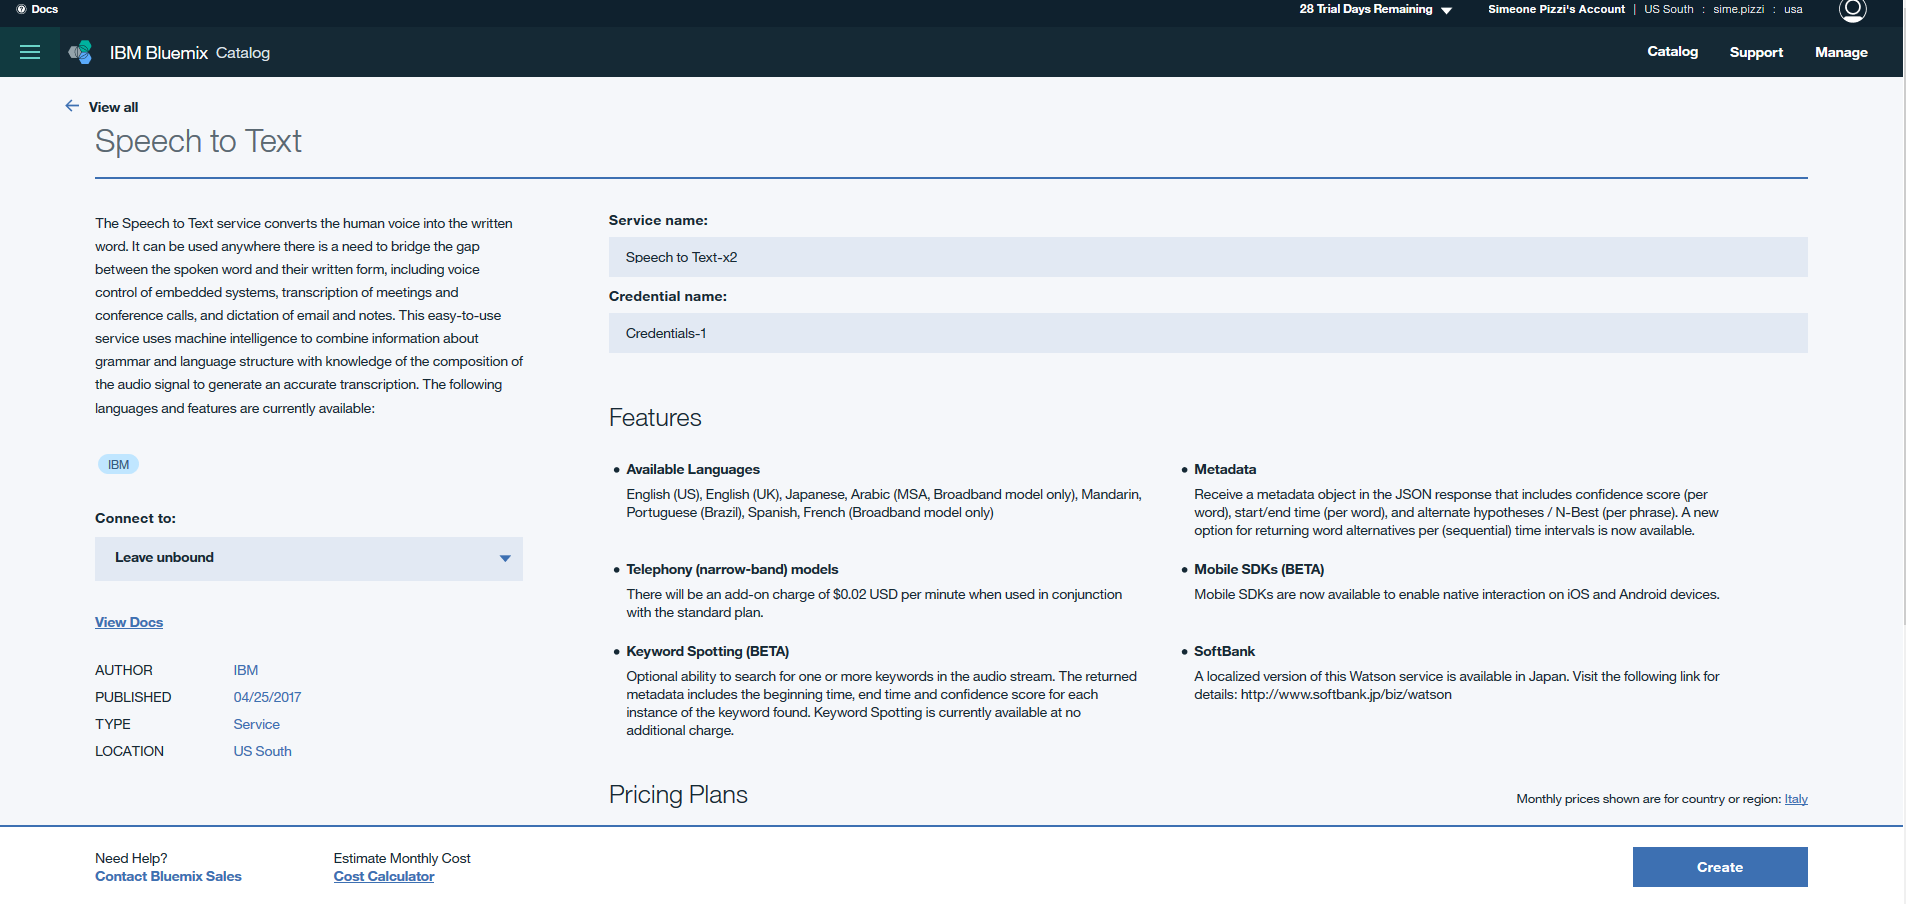
\includegraphics[width=1\textwidth,height=\textheight,keepaspectratio]{sezioni/images/watson-create.PNG}}
	\caption{Creazione del servizio di STT in IBM Watson}\label{fig:serviceWatson}
\end{figure}
\begin{figure}[h]
	\centerline{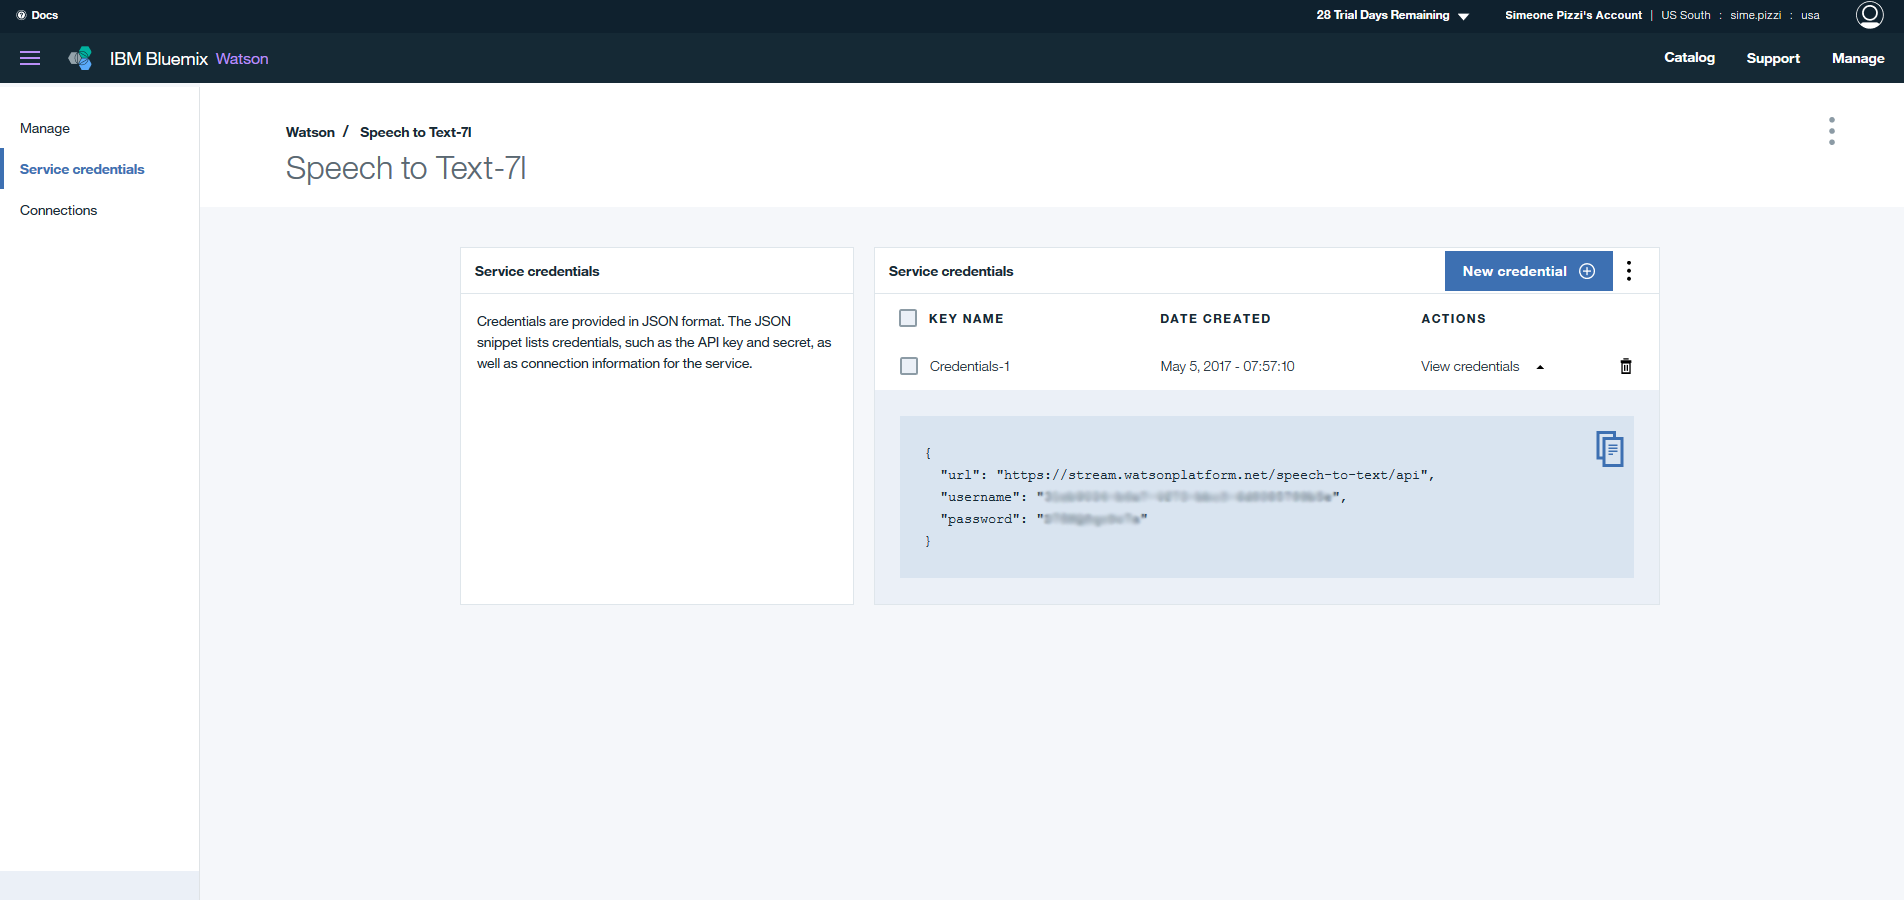
\includegraphics[width=1\textwidth,height=\textheight,keepaspectratio]{sezioni/images/watson-credentials.PNG}}
	\caption{Visualizzazione delle credenziali di STT in IBM Watson}\label{fig:credentialsWatson}
\end{figure}
\newpage
\subsubsection{api.ai}
\paragraph{Creazione}
È il Software Development Kit (SDK) utilizzato per l'effettiva costruzione dell'assistente virtuale.
È necessario creare un account al link \url{https://api.ai/} (visitato in data 2017-05-02) cliccando sul pulsante "sign up free", ma se si dispone già di un account Google, Facebook, Slack o Github è possibile effettuare l'accesso tramite uno di essi cliccando sul pulsante "log in".
\begin{figure}[h]
\centering{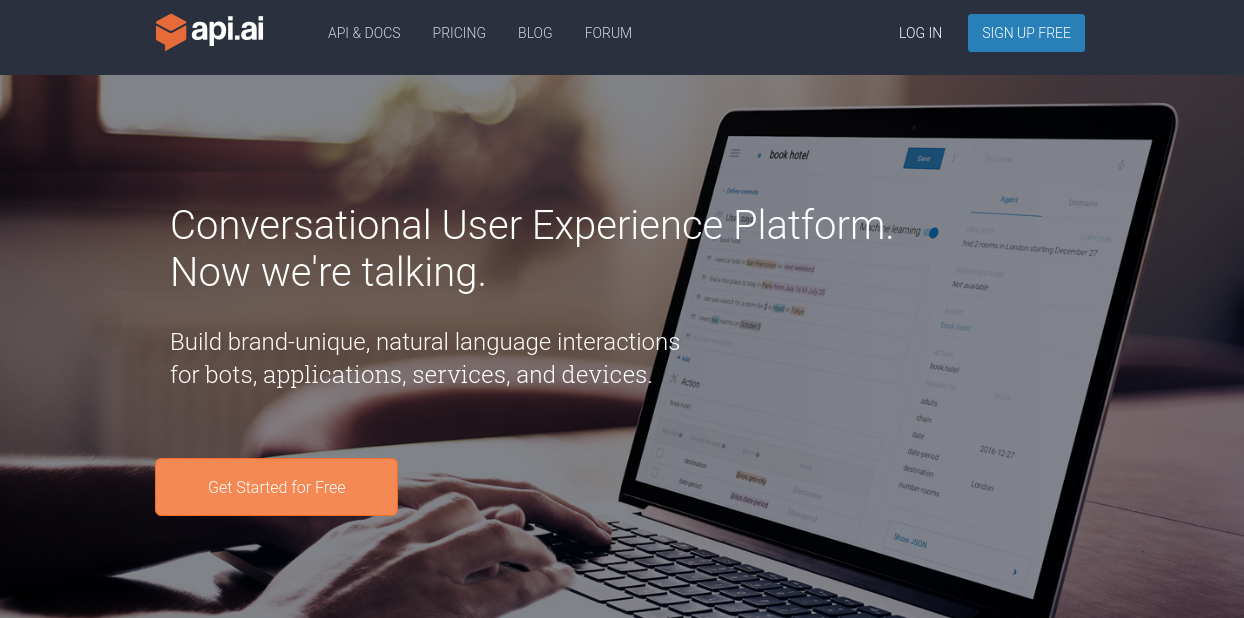
\includegraphics[width=0.7\textwidth,height=\textheight,keepaspectratio]{sezioni/images/apiai.png}}
	\caption{Registrazione api.ai}
\end{figure}
\newpage
\paragraph{Configurazione}
Dopo aver effettuato l'accesso, selezionare il menù degli \gl{agent} a sinistra (figura \ref{fig:menuapi}) e scorrerlo fino in fondo, selezionando "Create new agent" (figura \ref{fig:newAgent}). \\

Inserire nell'apposita schermata (figura \ref{fig:saveAgent}) i seguenti dati:
\begin{itemize}
	\item \textbf{Agent name}: ConversationAppGuest;
	\item \textbf{Agent type}: Private;
	\item \textbf{Language}: English;
	\item \textbf{Default time zone}: (GMT+1:00) Europe/Rome.
\end{itemize}
Cliccare poi "SAVE".
Successivamente, è necessario importare il primo agent applicando la seguente procedura:
\begin{itemize}
	\item selezionare l'agent appena creato nel menù a sinistra (figura \ref{fig:menuapi});
	\item cliccare il simbolo dell'ingranaggio, successivamente la voce "Export and Import" ed infine il pulsante "Import from zip" (figura \ref{fig:importAgent});
	\item l'agent da importare si trova nel repository scaricato (\ref{download}) in\\ \file{AtAVi/src/Back-end/VirtualAssistant/ApiAi/ConversationAppGuest}
\end{itemize}


Creare un secondo agent, chiamato "ConversationAppAdmin" e con percorso\\ \file{AtAVi/src/Back-end/VirtualAssistant/ApiAi/ConversationAppAdmin}, seguendo le istruzioni appena esposte.
\begin{figure}[h]
	\centering{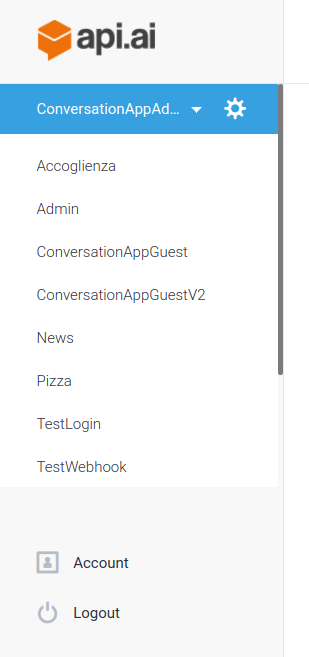
\includegraphics[width=0.3\textwidth,height=\textheight,keepaspectratio]{sezioni/images/menuapi.png}}
	\caption{menu agent api.ai}\label{fig:menuapi}
\end{figure}
\begin{figure}[h]
	\centering{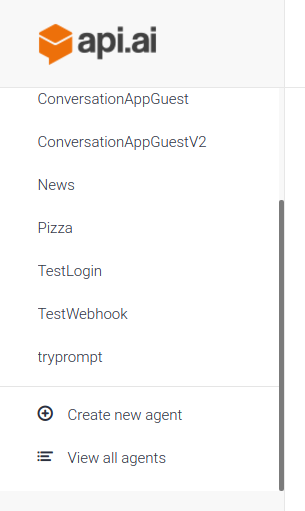
\includegraphics[width=0.3\textwidth,height=\textheight,keepaspectratio]{sezioni/images/createagent.png}}
	\caption{nuovo agent api.ai}\label{fig:newAgent}
\end{figure}
\begin{figure}[h]
	\centering{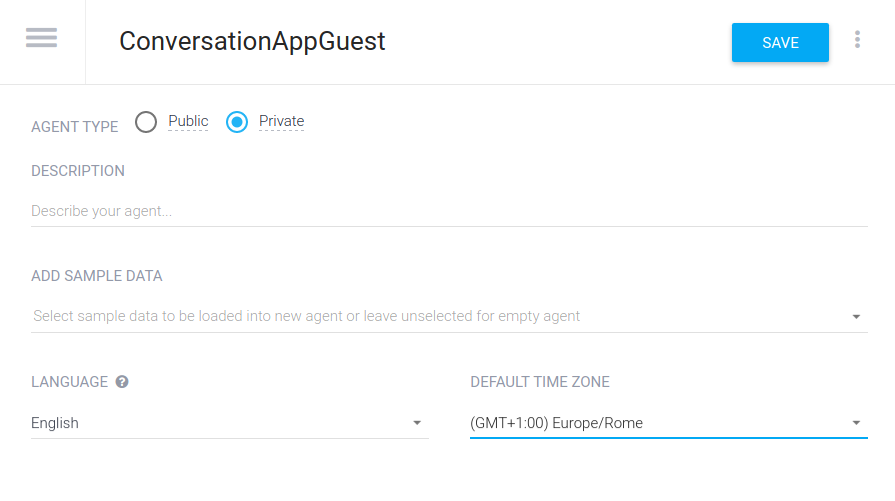
\includegraphics[width=0.7\textwidth,height=\textheight,keepaspectratio]{sezioni/images/saveagent.png}}
	\caption{save agent api.ai}\label{fig:saveAgent}
\end{figure}
\begin{figure}[h]
	\centering{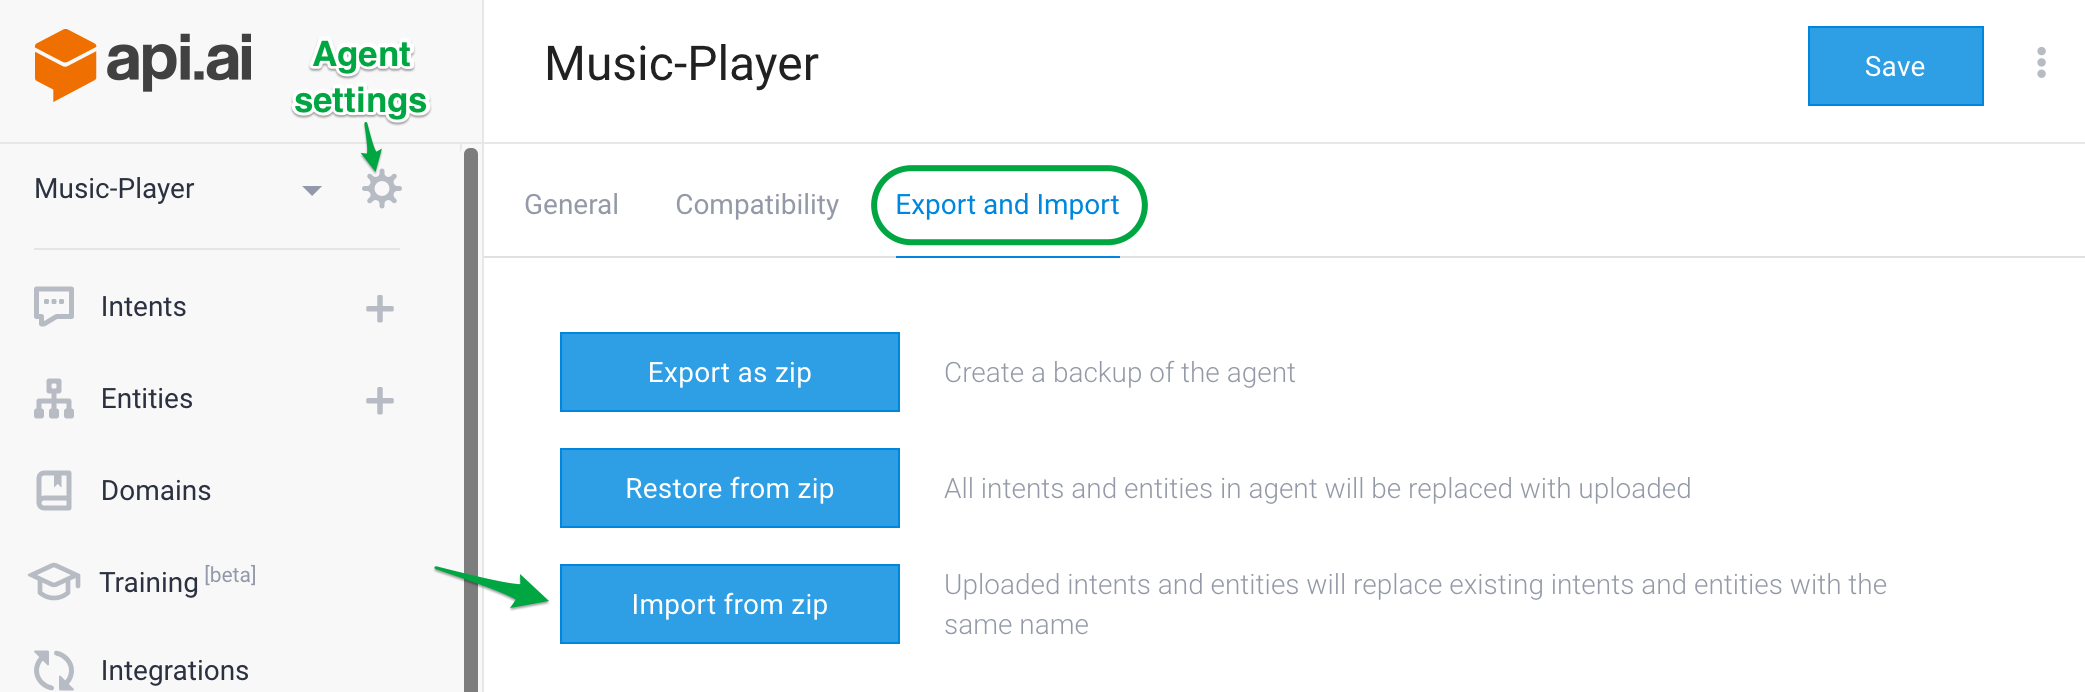
\includegraphics[width=1\textwidth,height=\textheight,keepaspectratio]{sezioni/images/importagent.png}}
	\caption{import agent api.ai}\label{fig:importAgent}
\end{figure}


\subsection{Deploy}
Una volta completate le procedure descritte in \ref{download} e \ref{configurazione}, si può procedere al deploy dei microservizi, dell'API Gateway, del Topic SNS e delle Lambda Function create.\\Riportiamo in seguito la lista delle operazioni da eseguire in ordine per un corretto deploy.  

\subsubsection{Installazione moduli npm}
Per ottenere i moduli npm necessari al corretto funzionamento del prodotto è sufficiente recarsi da terminale nella cartella root del prodotto e lanciare il comando \file{npm install}.

\subsubsection{Compilazione}
Per la compilazione del codice viene utilizzato Grunt. Per poter usufruire di tale servizio è necessario recarsi nella cartella root del prodotto e lanciare il comando \file{npm install -g grunt}.
Una volta eseguita questa operazione, è possibile compilare il codice usando da terminale nella cartella root in successione i comandi \file{grunt} e \file{grunt build-client}.

\subsubsection{Deploy dei microservizi}
Una volta completata l'installazione dei moduli e la compilazione, è possibile eseguire il deploy dei microservizi. Per il microservizio Notifications prima di eseguire il deploy è necessario inserire nel file \file{AtAVi/dist/Back-end/Notifications/secret.yml} il token ottenuto dalla creazione del bot Slack, come spiegato nella sezione ??????????????.
In seguito, è sufficiente dare il comando \file{sls deploy} (oppure \file{serverless deploy}) con il terminale aperto, in ordine, nelle seguenti cartelle:
\begin{itemize}
	\item \file{AtAVi/dist/Back-end/VirtualAssistant};
	\item \file{AtAVi/dist/Back-end/Notifications};
	\item \file{AtAVi/dist/Back-end/Rules};
	\item \file{AtAVi/dist/Back-end/Users}.
\end{itemize}
Per ognuno dei deploy appena eseguiti, il terminale restituirà una API-key e gli URL degli endpoints che serviranno per il deploy delle componenti successive.

\subsubsection{Deploy dei webhook}
Una volta eseguito il deploy dei microservizi è necessario eseguire il deploy dei webhook. Prima di eseguire il deploy di AdministrationWebhookService è necessario  inserire nel file \file{AtAVi/dist/Back-end/AdministrationWebhookService/secret.yml} la chiave utilizzata per criptare il token JWT. Successivamente è possibile eseguire i deploy dando il comando \file{sls deploy} (oppure \file{serverless deploy}) con il terminale aperto, in ordine, nelle seguenti cartelle:
\begin{itemize}
	\item \file{AtAVi/dist/Back-end/AdministrationWebhookService};
	\item \file{AtAVi/dist/Back-end/ConversationWebhookService};
	\item \file{AtAVi/dist/Back-end/CuriosityWebhookService}.
\end{itemize}

\subsubsection{Deploy di Events}
Per il deploy di Events è necessario inserire nel file \file{AtAVi/dist/Back-end/Events/secret.yml} le seguenti informazioni:
\begin{itemize}
	\item ARN del Topic SNS;
	\item URL e API-key del microservizio Rules;
	\item URL e API-key del microservizio Notifications;
	\item canale di default Slack (ottenuto nella sezione ?????).
\end{itemize}
È ora possibile eseguire il deploy di Events, dando il comando \file{sls deploy} (oppure \file{serverless deploy}) con il terminale aperto nella cartella: \file{AtAVi/dist/Back-end/Events}.


\subsubsection{Deploy di APIGateway}
Per il deploy di APIGateway è necessario inserire nel file \file{AtAVi/dist/Back-end/APIGateway/secret.yml} le seguenti informazioni:
\begin{itemize}
	\item URL e API-key del microservizio Rules;
	\item URL e API-key del microservizio Users;
	\item URL e API-key del microservizio VirtualAssistant;
	\item key di Azure ottenuta come spiegato nella sezione ???????;
	\item id dell'account Amazon ottenuto come spiegato nella sezione ??????;
	\item username e password del servizio IBM Watson STT ottenuti come spiegato nella sezione ?????????;
	\item chiave utilizzata per criptare il token JWT.
\end{itemize}
Si prosegue ora col deploy di APIGateway, dando il comando \file{sls deploy} (oppure \file{serverless deploy}) con il terminale aperto nella cartella: \file{AtAVi/dist/Back-end/APIGateway}.

\subsubsection{Collegamento dei piani d'uso con le API-key}





\newpage

